%\addbibresource{/home/jorgsk/phdproject/bibtex/jorgsk.bib}

%What results should you present? Anything more than was presented in the paper?

%The figure with the compartments and poly(A)-.

%Shows two things: 1) there is poly(A) signal in poly(A)- extract. explained by
%errors in screening and possibly by short poly(A). 2) intronic polyadenylation in the nucleus overrepresented. Makes
%sense if there is nuclear degradation of intronic poly(A) which has been
%recently shown.

%Then the figure with overlap to show how much you get?

%Then the figure that shows the flattening out of the getting of new
%transcripts.

%Discuss each of the tree figures and that's it.

%Maybe make a table with some of the numbers from the statistics you output.

%Then cite the paper.
\subsection{Summary of the paper}
Summarize the paper.

\subsection{The dataset}
The datasets used in this study were generated by the ENCODE
(\textbf{Enc}yclopedia \textbf{O}f \textbf{D}NA \textbf{E}lements) consortium
and are available from http://hgdownload-test.cse.ucsc.edu/goldenPath/hg19/encodeDCC/wgEncodeCshlLongRnaSeq/

The data is from RNA-seq experiments from 12 human cell lines. Six of the cell
lines have RNA-seq data from whole cell extracts and the remaining six cell
lines have RNA-seq data from cytoplasmic and nuclear extracts in a addition to
the whole cell. Each cell line is further available in both the poly(A)+ and
poly(A)- fractions of the RNA pool. Table \ref{tab:Datasets} shows the cell
lines and compartments used; as can be seen, most experiments were available
with a biological replicate. In total, 23 datasets were from whole cell
extracts, 11 were from cytoplasmic extracts, and 12 were from nuclear extracts.
This brings the total to 92 RNA-seq datasets. The datasets contains only
RNA-seq from long RNA, defined as RNA over 200 nucleotides in length. Each
dataset has been generated with Illumina paired-ended sequencing with a
read-length of 75 basepairs. Each dataset contains between 150 and 250 million
reads.

\begin{table}
	\centering
	\begin{tabular}{cccc}
	  Cell line & Whole Cell & Cytoplasm & Nucleus \\
	  \midrule
	  GM12878 & 2 & 2 & 2 \\
	  K562 & 2 & 2 & 2 \\
	  HeLa-S3 & 2 & 2 & 2 \\
	  HUVEC & 2 & 2 & 2 \\
	  HEPG2 & 2 & 2 & 2 \\
	  H1Hesc & 1 & 1 & 1 \\
	  Nhek & 2 & 0 & 1 \\
	  MCF7 & 2 & 0 & 0 \\
	  AG04450 & 2 & 0 & 0 \\
	  HSMM & 2 & 0 & 0 \\
	  NHLF & 2 & 0 & 0 \\
	  A549 & 2 & 0 & 0 \\
	\end{tabular}
	\caption{Number of replicates of the datasets from the ENCODE consortium}
	\label{tab:Datasets}
\end{table}

What sets this library apart from most RNA-seq data is that the cell is
compartmentalized and that both the poly(A)+ and poly(A)- fractions of RNA have
been sequenced separately; these extra dimensions increase the resolution of
the data, allowing new hypothesises to be asked. The poly(A)+ fraction of
an RNA sample contains all the RNA that is captured by a poly(T) primer column.
This will include all processed mRNA with a poly(A) tail of more than 20
nucleotides (the length of the poly(T) primer). The poly(A)- fraction is the
complement of the poly(A)+ fraction and contains mostly noncoding RNA and
pre-processed mRNA.

\subsection{The short RNA mapper}
The short read mapper used in this work is the GEM mapper
\cite{ribeca_gem_2010}. The GEM mapper is developed in the group of Roderic
Guigo and is production ready, although it has not been published yet.

\subsection{The PET data}
Another technique for locating the 3\p end of a transcript is by Paired End
diTag (PET) Sequencing. This technique adds two tags to the 3\p end and the
5\p end of an RNA. Those tags then join with each other, forming a circular
RNA. Later, only the sequences close to the two tags are sequenced. Thereby,
one obtains the sequence information both about both the transcription start
site and the transcript termination site of the RNA. By mapping those sequences
back to the genome, it is possible to find out where the RNA began and ended.
We have used PET data developed by ENCODE which is available from
http://hgdownload.cse.ucsc.edu/goldenPath/hg19/encodeDCC/wgEncodeGisRnaPet/ to
compare with the polyadenylation sites we discovered using Utail. We demanded a
coverage of 10 PET reads to accept a site as transcript termination site.

\section{Results}
We developed a software called Utail and ran it on the ENCODE RNA-seq data.
For details on how Utail works, see the Appendix. Parts of the analysis from
Utail's output was published in Djabeli et al. XXX. The description of the
methods we used are found in the supplementary materials of the paper by
Djabeli et al. and in the Appendix. Briefly, the method involves mapping
polyadenylation sites onto the genome and clustering them if they are within 20
nucleotides of each other, since this is close to the maximal range of the
stochastic effect of choice of 3\p cleavage site \cite{tian_large-scale_2005}.
After clustering we search the genomic sequence 40 nucleotides downstream the
polyadenylation site for one of the polyadenylation signals (PAS). Finally we
intersect the polyadenylation sites with the 3\p PET sites to see which
overlap.

Now we will describe the parts of the analysis that was not included in paper.

\subsection{Total number of polyadenylation sites}
By merging all polyadenylation sites from all datasets, we identified a total
of 158.000 polyadenylation sites in the genome for the poly(A)+ fraction and
86000 polyadenylation sites for the poly(A)- fraction. Figure
\ref{fig:saturation} shows how the number of new polyadenylation sites
saturates as the number of datasets increases. The saturation is sharper for
polyadenylation sites which have are annotated with a downstream PAS. Since a
downstream PAS is commonly found in polyadenylation sites, this is a signal
that the number of false positives increases when the number of clustered reads
becomes very large. 

\subsection{Distribution of polyadenylation sites across the genome}
We found that most of the polyadenylation sites are in the 3\p UTR exonic
regions, as expected, but there are also many polyadenylation sites in the
intergenic and intronic regions as well, see Figure \ref{fig:sidebars}. In the
poly(A)+ fraction, there is more intronic poly(A) sites in the nucleus than in
the cytoplasm. This can partially be expected since most introns are removed in
the nucleus. Some introns however are included in the final mRNA, and some
contain poly(A) sites \cite{tian_widespread_2007}. The whole cell is as
expected an average between the nuclear and cytoplasmic compartments.

We also found evidence for polyadenylated RNA in the poly(A)- fraction, see
Figure \ref{fig:sidebars} B. This was unexpected, since the poly(A)- fraction
is supposed by design not to contain RNA with poly(A) tails. We surmised that
the polyadenylated RNA in the poly(A)- fraction could have three possible
sources. Source one (S1) is normal poly(A)+ mRNA with full length poly(A) tails
that did not get absorbed by the poly(A)+ filtration step and thus ended up in
the poly(A)- fraction. Source two (S2) is mRNA with poly(A) tails shorter than
20nt; either they have had their polyA tails degraded to below 20 nucleotides,
or they were actively undergoing polyadenylation at the time of sampling and
did not reach a poly(A) tail length of more than 20 nucleotides. Source three
(S3) are RNA with short, degradation-related transient poly(A) tails which have
been identified in the nucleus of mammalian cells \cite{lemay_nuclear_2010}.

\subsection{Isolating polyadenylation sites unique to the poly(A)- and poly(A)+
fractions}
We wanted to separate the S3 from the S1 and S2 poly(A) sites. We did this by
recognizing that many of the S1 and S2 sites are likely to be present in both
the poly(A)- and the poly(A)+ fractions, since these sites really belong to
poly(A)+ transcripts that have accidentally ended up in the poly(A)- fraction.
Therefore, we filtered out all the poly(A) sites that intersected the poly(A)+
and poly(A)- fraction and removed these from both fractions. As can be see in
in Figure \ref{fig:sidebars_intersect}, almost no poly(A) sites remain in the
poly(A)- fraction of the cytoplasm. And while the nuclear poly(A)- fraction
lost many of the polyadenylation sites in the 3UTR exonic region, the number
sites in intergenic and intronic regions did not change by much.

We believe that the enrichment of the poly(A)- poly(A) sites in the nuclear
fraction in general is due to degradation-related transient polyadenylation
that occurs in the nucleus of mammalian cells \cite{lemay_nuclear_2010,
lacava_rna_2005, wyers_cryptic_2005}. In the nuclear compartment, the intronic
region stands out, but part of this is due to the fact that introns comprise a
large part of nuclear RNA, since human pre-mRNA sequences contain over 20 times
more intronic than exonic sequence \cite{venter_sequence_2001}.

\begin{figure}[htb]
	\begin{center}
		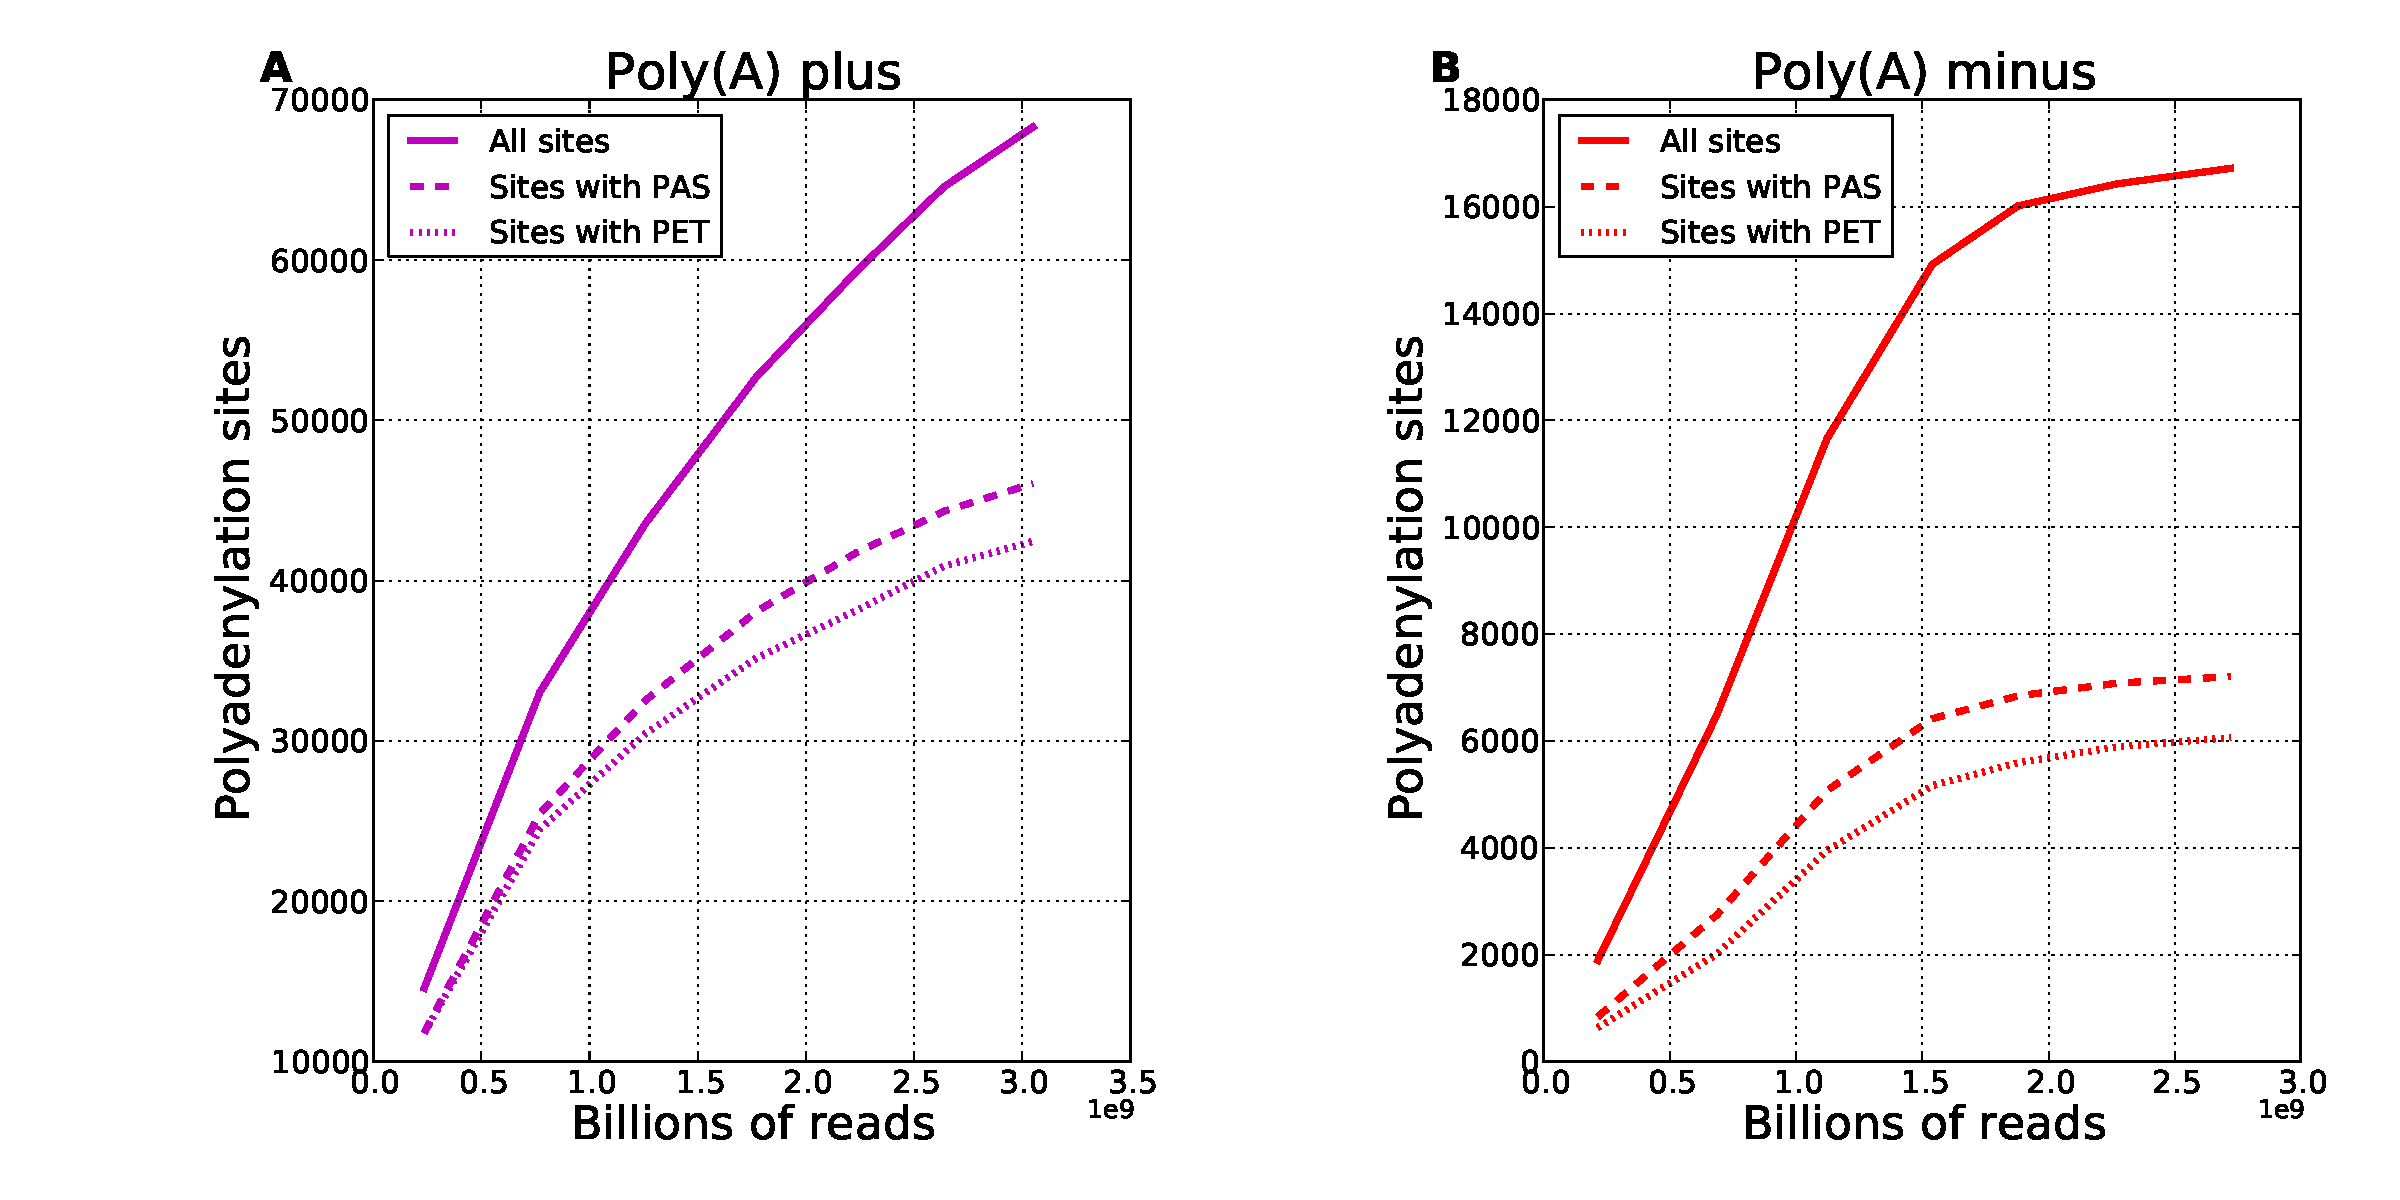
\includegraphics[scale=0.3]{figures/polyadenylation/Saturation_plot_2+.pdf}
	\end{center}
	\caption{Saturation of discovery of polyadenylation sites}
	\label{fig:saturation}
\end{figure}

\begin{figure}[htb]
	\begin{center}
		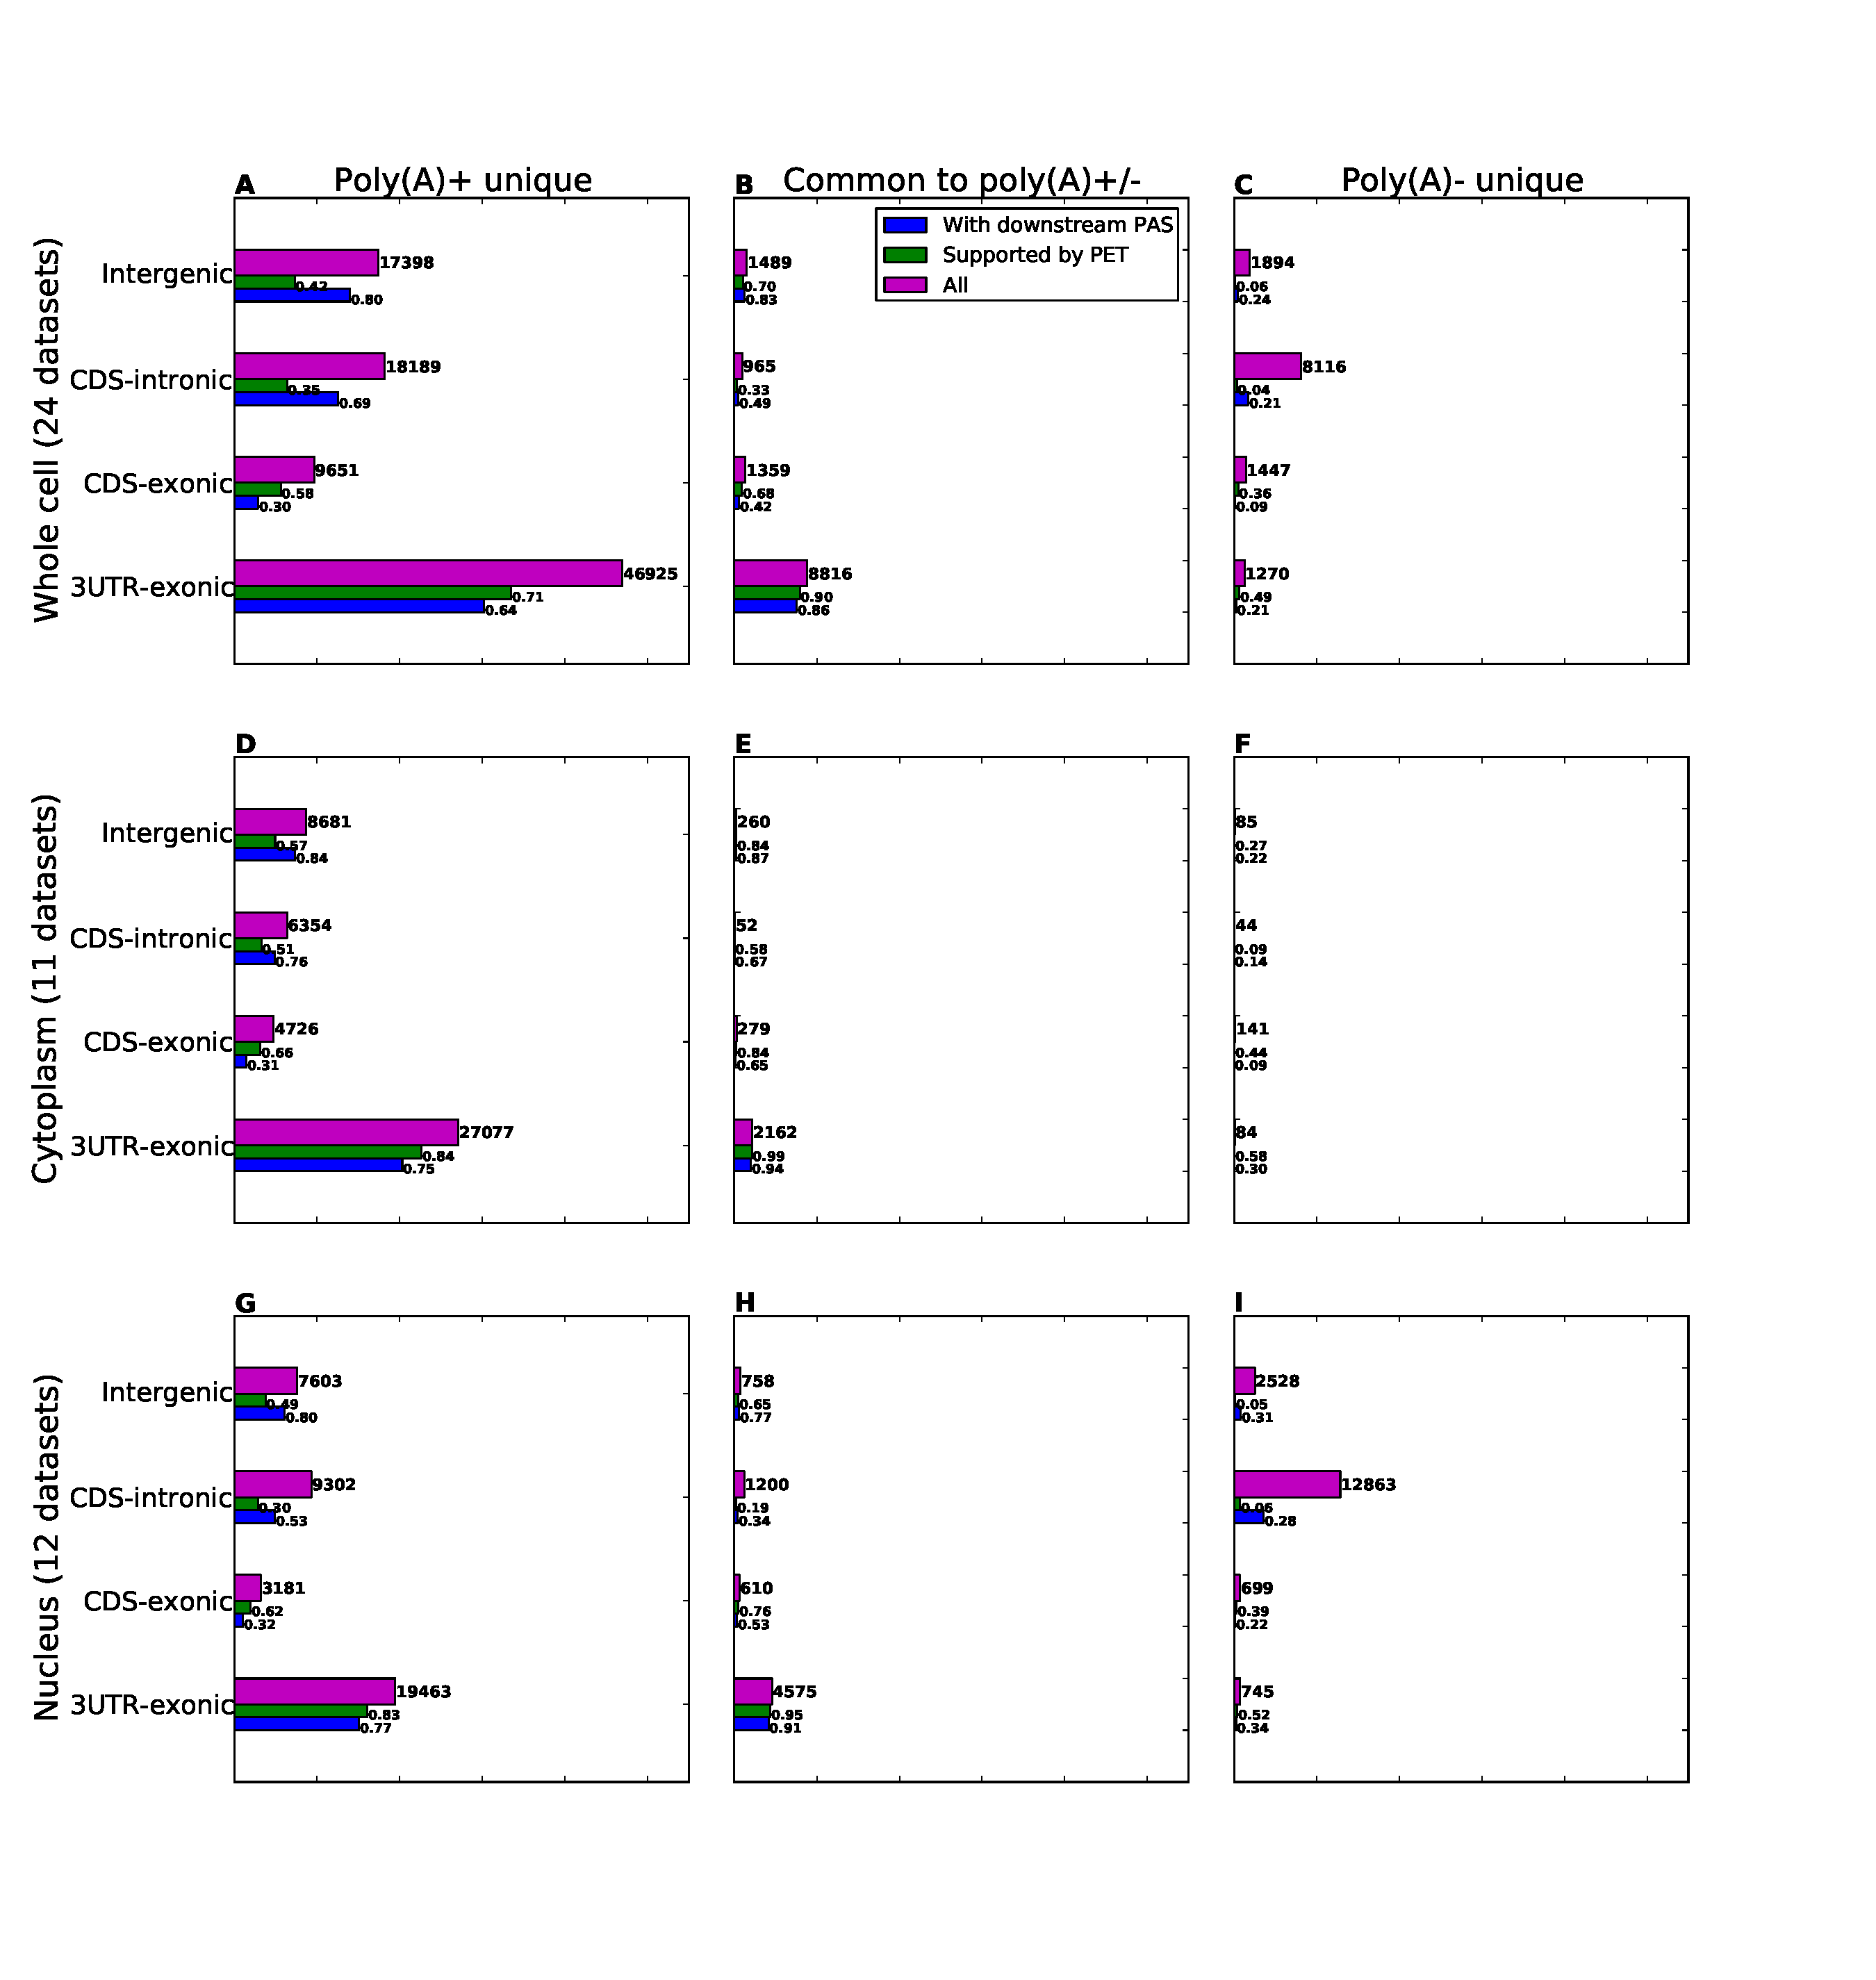
\includegraphics[scale=0.3]{figures/polyadenylation/intersected_sidebars_pA_2+.pdf}
	\end{center}
	\caption{Polyadenylation across genomic regions for the poly(A)+ and poly(A)-
	fractions and the sites that overlap the poly(A)+ and poly(A)- fractions}
	\label{fig:sidebars_intersect}
\end{figure}

\begin{figure}[htb]
	\begin{center}
		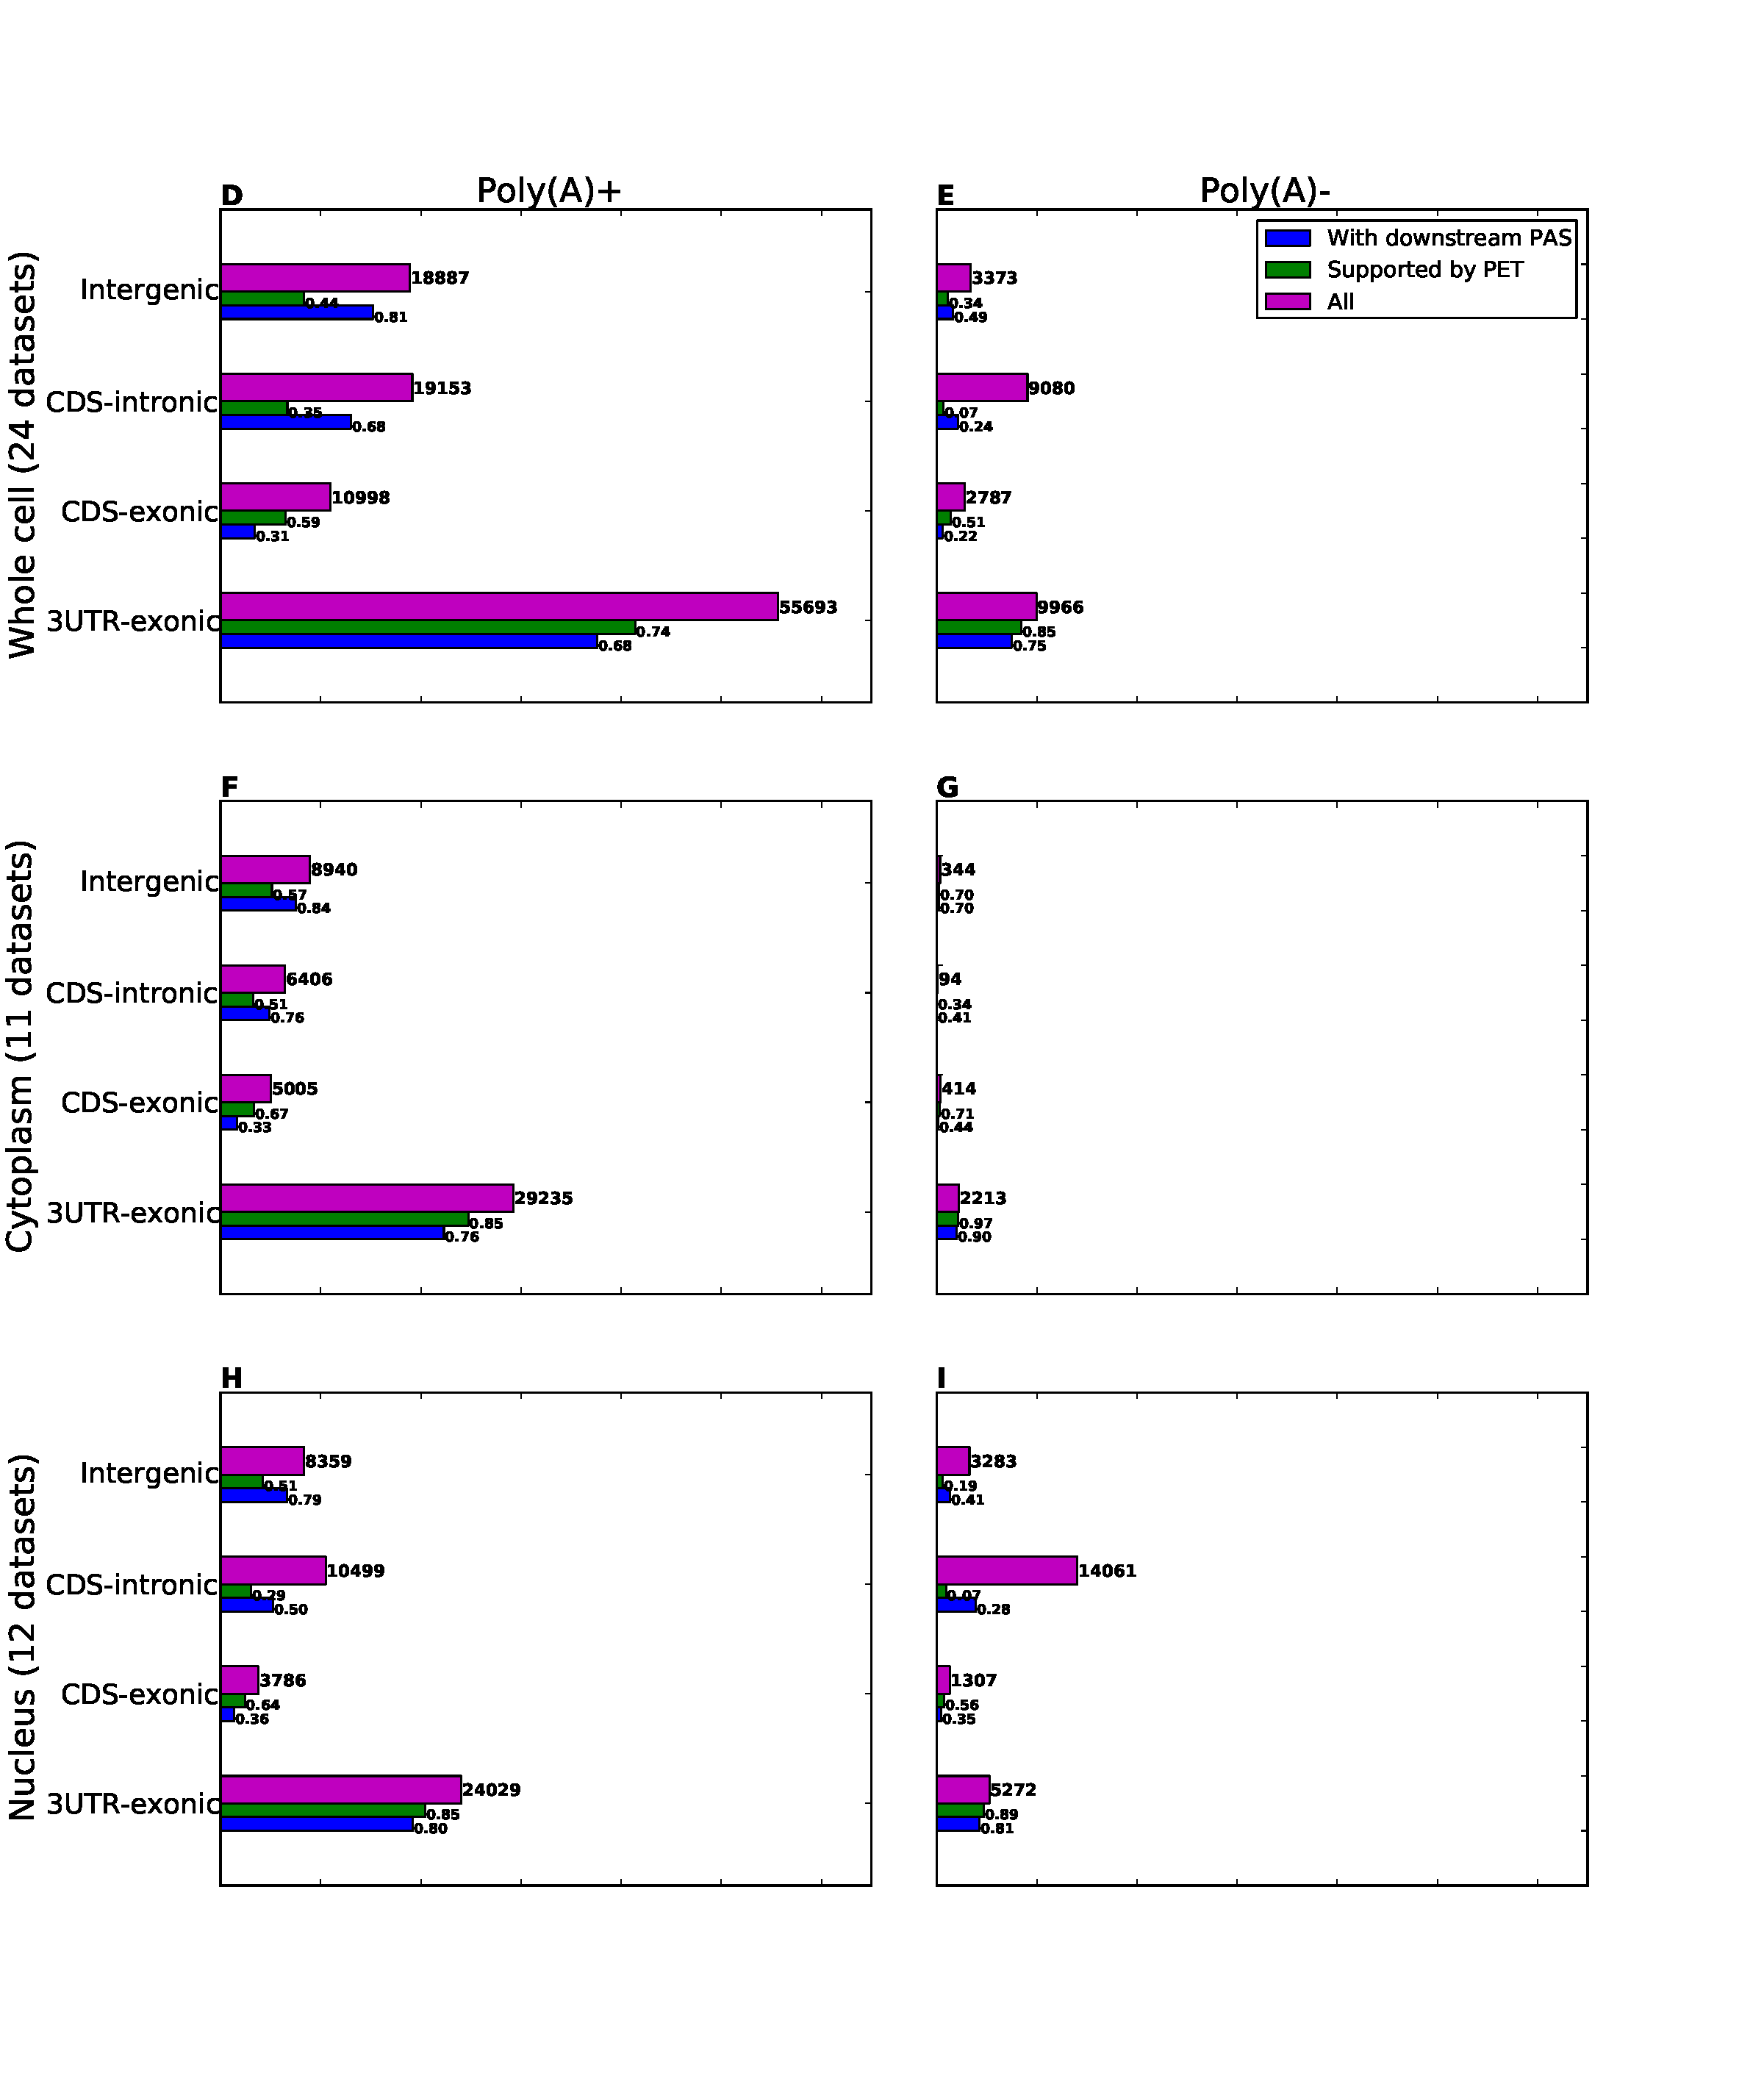
\includegraphics[scale=0.4]{figures/polyadenylation/Sidebars_pA_2+.pdf}
	\end{center}
	\caption{Polyadenylation across genomic regions for the poly(A)+ and poly(A)-
	fractions}
	\label{fig:sidebars}
\end{figure}

\subsubsection{Discussion}
The polyadenylation in intergenic regions indicate either unannotated long 3\p
UTR ends or cleavage and polyadenylation sites of novel transcripts.
